% Metódy inžinierskej práce

\documentclass[10pt, twoside, slovak,a4paper]{article}
\usepackage[slovak, english]{babel}
\usepackage[IL2]{fontenc} 
\usepackage[utf8]{inputenc}
\usepackage{graphicx}
\usepackage{url}
\usepackage{hyperref} 
\graphicspath{{imgs/}}
\usepackage{cite} 
\usepackage{tabularx}
\newlength\tindent
\setlength{\tindent}{\parindent}
\setlength{\parindent}{0pt}
\renewcommand{\indent}{\hspace*{\tindent}}



\pagestyle{headings}

\title{Describing the capabilities and cases of uses for sequence diagrams in software engineering \thanks{Semestrálny projekt v predmete Metódy inžinierskej práce, ak. rok 2021/22, vedenie: Shevchenko Serhii}} % meno a priezvisko vyučujúceho na cvičeniach

\author{Shevcheko Serhii\\[2pt]
	{\small Slovenská technická univerzita v Bratislave}\\
	{\small Fakulta informatiky a informačných technológií}\\
	{\small \texttt{xshevchenko@stuba.sk}}
	}

\date{\small 14. december 2021} 



\begin{document}

\maketitle

\begin{abstract}
The article will describe the general principles of constructing sequence diagrams, and provide optimal cases of their use in the field of software engineering modeling.

The main structural elements of a sequence diagram will be described, the rules for their use with corresponding examples.
\end{abstract}



\section{Introduction}

In the well-known graphical description language for modeling in the field of software development, UML, there are several types of diagrams, each of which has its own advantages and disadvantages.

Among the popular types of diagrams are class diagrams, component diagrams, and activity diagrams.

The problem with all the above diagrams is that they cannot simulate the dynamics of the model, the behavior and the relationship between "actors" over time. They represent the structure, but not the behavior of the model on the timeline.

To solve this problem, a sequence diagram was created. It, unlike other types of diagrams, shows the interactions of "actors" on the timeline, the exchange of "messages" (data) between them. And, again, this is all shown in projection on the time axis. That is, it allows to explore the model in dynamics~\cite{Sequence_diagram:Lambert}.

\section{What is UML} \label{what_is_diagram}

Before we talk about sequence diagrams, we should first understand what UML is, of which the sequence diagram is a part.

The Unified Modeling Language (UML) is a general-purpose, developmental, modeling language in the field of software engineering that is intended to provide a standard way to visualize the design of a system~\cite{UML_Distilled}. 

In other words, we can say that UML is a set of rules and recommendations on how to create visual structural and relational models of software systems.

The creation of UML was originally motivated by the desire to standardize the disparate notational systems and approaches to software design. It was developed at Rational Software in 1994–1995, with further development led by them through 1996~\cite{UML_user_guide:Booch}.

\subsection{What UML include}

The fact is UML consist of many types of diagrams \ref{UML:diagrams}. In order to understand the benefits of a sequence diagram, it is important first to understand what other diagrams exist in UML and for what purposes they are used.

\begin{figure*}[tbh]
	\centering
	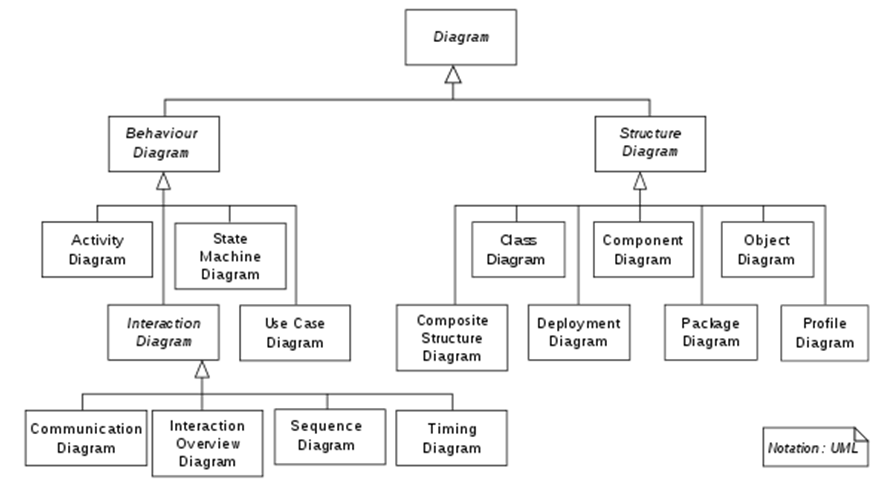
\includegraphics[scale=0.5]{UML diagrams.png}
	\caption{Diagram types \cite{UML_user_guide:Booch}.}
	\label{UML:diagrams}
	\end{figure*}

Looking at Figure \ref{UML:diagrams}, we see that the structural tree of UML diagrams is rather voluminous. Not all of these diagrams are actively used in the development industry ~\cite{UML_Distilled}, but each was created for a specific purpose. In Table \ref{Table}, we can see the 4 main types of diagrams actively used in the development industry, and a short summary of their purpose and structural composition.

 \begin{table}[htbp]
	\begin{tabular}{|p{0.35\linewidth}|p{0.35\linewidth}|p{0.35\linewidth}|}
	\hline
					  & Uses for representation                                                          & Consist of                                    \\ 
					  \hline
	Sequence diagram  & relations of the object in time sequence                                         & objects and messages on lifeline.             \\ 
	\hline
	Class diagram     & static classes structure in a model and relations between them.                  & classes, that contain attributes and methods. \\ 
	\hline
	Activity diagram  & of workflows of stepwise activities and actions.                                 & activities and logic blocks.                  \\ 
	\hline
	Component diagram & how components are wired together to form larger components or software systems. & structural components.                        \\ 
	\hline
	\end{tabular}
	\caption{Main diagrams qualities\cite{UML_Distilled}.}
	\label{Table}
\end{table}

It can be concluded that all 4 types of diagrams are completely different and are used for different purposes. Thus, it is possible to understand how UML is a universal tool for building systems models.

\section{When to use a sequence diagram} \label{when}

A sequence diagram should be used primarily to visualize relationships between objects, taking into account the sequence of these very relationships~\cite{IBM_SD}.

This diagram is very useful for modeling synchronous services, it allows thinking through all the interactions between "actors" from the beginning to the end of the service life cycle on the timeline.

An organization’s technical staff can find sequence diagrams useful in documenting how a future system should behave. During the design phase, architects and developers can use the diagram to force out the system’s object interactions, thus fleshing out overall system design.

One of the primary uses of sequence diagrams is in the transition from requirements expressed as use cases to the next and more formal level of refinement. Use cases are often refined into one or more sequence diagrams. In addition to their use in designing new systems, sequence diagrams can be used to document how objects in an existing (call it “legacy”) system currently interact\cite{Sequence_diagram:Lambert}.
\section{The notation} \label{notation}

\subsection{Frame} \label{notation:frame}

The first notation element to know is the frame. It is makes a graphical boundary of a sequence diagram and provide place for a diagram label (Frame \ref{fig:frame}).

In addition to providing a visual border, the frame element also has an important functional use in diagrams depicting interactions, such as the sequence diagram. On sequence diagrams incoming and outgoing messages (interactions) for a sequence can be modeled by connecting the messages to the border of the frame element.
\begin{figure*}[tbh]
\centering
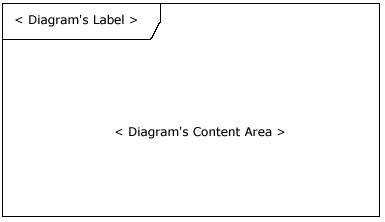
\includegraphics[scale=0.35]{frame.jpg}
\caption{Frame template \cite{Sequence_diagram:Lambert}.}
\label{fig:frame}
\end{figure*}

This element is not required in sequence diagrams, but it is better to use it for convenience. When using this element, it is necessary to place all subsequent elements, which will be described below, inside the frame.

\subsection{Lifelines} \label{notation:lifelines}
When drawing a sequence diagram, lifeline notation elements are placed across the top of the diagram.

Lifelines are designations of objects that make up the model, and between which information is exchanged. This is one of the key elements of a sequence diagram.
\begin{figure*}[tbh]
	\centering
	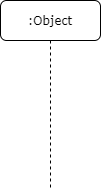
\includegraphics[scale=0.4]{lifeline.png}
	\caption{Lifeline template \cite{Sequence_diagram:Lambert}.}
	\label{fig:lifeline}
\end{figure*}

Lifelines are drawn as a box with a dashed line descending from the center of the bottom edge (Figure \ref{fig:lifeline})\cite{IBM_SD}.


\subsection{Messages} \label{notation:messages}
Messages are illustrating calling a function from one object to another, data exchange between the objects.
\begin{figure*}[tbh]
	\centering
	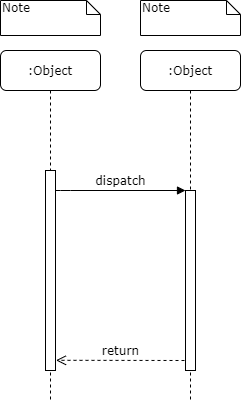
\includegraphics[scale=0.4]{Message.png}
	\caption{Messages template \cite{Sequence_diagram:Lambert}.}
	\label{fig:messages}
\end{figure*}
There are dispatch messages, that display calling functions, and return message, that display end of execution\cite{UML}.

White rectangle is an Execution Specification, it is used to visually display the start and end of an operation.
\section{Building a Sequence Diagram} \label{building}

Consider the construction of a sequence diagram using figure \ref{fig:sd_example} as an example. This is an example of a simple user registration system. First, the client fills in the registration form by accessing the UI of the system. After that, a request to save the user is sent. A check is made to see if the user exists in the system. If yes, an error message is returned. If no - the success message is shown.

\begin{figure*}[tbh]
	\centering
	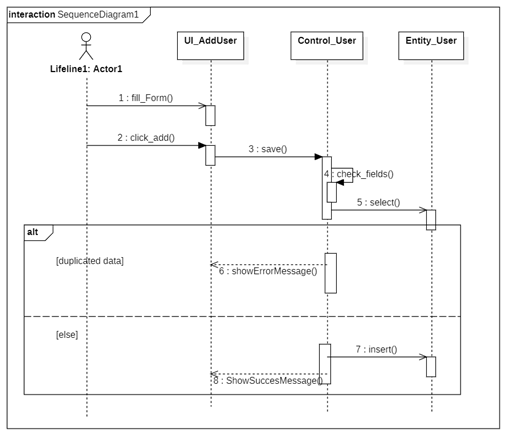
\includegraphics[scale=0.7]{Sequence Diagram Example.png}
	\caption{Sequence diagram example \cite{System_analys:Dennis}.}
	\label{fig:sd_example}
\end{figure*}

This example allows you to understand how message passing works, which in this context are calls of necessary functions in the desired object, the sequential execution of these functions. It should be noted that this example perfectly illustrates how easy it is to use a sequence diagram to simulate the sequence of actions in the system.

\section{Conclusion} \label{Conclusion} 
This article described general information about UML diagrams. The most commonly used types of diagrams have been considered. It also described what are sequence diagrams. It was told about their notation. The structural elements of sequence diagrams were considered, and an example of building a sequence diagram was given.\\
\subsection{Response to topics from lectures}
\subsubsection{Engineering literacy and informatics}
An engineering-literate specialist has an understanding of the CDIO concept. It reveals an integral cycle of engineering activity - "invent - design - implement - manage".  Has primary experience of inventive activity in the development of new products and systems. Has the skill of situation analysis, solves production problems. 
He/she knows basic general scientific methods of knowledge (heuristic and logical), can apply them in other activities, knows special (private) mathematical methods and techniques, can apply them to solve mathematical and applied problems, has engineering culture of thinking, communication culture, working culture, has an idea about the main periods of science and technology development as components of human culture.
Thus, "engineering literacy" is a complex multi-component concept closely related to the concept of "functional literacy" in terms of future specialist's personality formation both within the framework of his/her professional and social experience.\\

\subsubsection{Internet in Educational and Business Environment}
The real implementation of the Internet in the educational process is determined by the extent to which its use is associated in the student's mind with future professional (independent) activities. 
Consequently, the introduction should begin with the organization of students' independent work on the basis of the Internet. 
The introduction of the Internet in the educational process changes the organization of students' independent work, which is based on information interaction of subjects of the educational process within the educational Internet environment, which provides greater independence of students, greater individualization of tasks. 
This work takes place outside class time, but due to the communication capabilities of network technologies, the student at any time can get the necessary advice, take part in the discussion of the problem, work on the project.\\ 

\subsubsection{Bibliography and citation in a technical text}
The list of references is an obligatory part of the scientific work and shows the listener's ability to apply in practice the knowledge received during the study of the relevant disciplines.
The list includes bibliographic information about the sources used in the preparation of the work.
It is also recommended to include bibliographical notes on cited in the text of the work documents and sources of factual or statistical information (in this case sublinear or intra-text bibliographical references are not formalized).
In works of retrospective or review character it is necessary to mention this or that edition. If the list includes bibliographic information about editions with which the listener was not directly acquainted, the bibliographic record specifies the source of information, from which the data about the edition were taken.\\

\bibliography{literatura}
\bibliographystyle{plain} 
\end{document}
